\documentclass[aspectratio=169%可调屏宽比16:9(169),4:3(43)
,serif,mathserif]{beamer}
\mode<presentation>{
%\usetheme{default}
%\usetheme{AnnArbor}
%\usetheme{Antibes}
%\usetheme{Bergen}
%\usetheme{Berkeley}
%\usetheme{Berlin}
%\usetheme{Boadilla}
%\usetheme{CambridgeUS}
%\usetheme{Copenhagen}
%\usetheme{Darmstadt}
%\usetheme{Dresden}
%\usetheme{Frankfurt}
%\usetheme{Goettingen}
%\usetheme{Hannover}
%\usetheme{Ilmenau}
%\usetheme{JuanLesPins}
%\usetheme{Luebeck}
\usetheme{Madrid}
%\usetheme{Malmoe}
%\usetheme{Marburg}
%\usetheme{Montpellier}
%\usetheme{PaloAlto}
%\usetheme{Pittsburgh}
%\usetheme{Rochester}
%\usetheme{Singapore}
%\usetheme{Szeged}
%\usetheme{Warsaw}
% As well as themes, the Beamer class has a number of color themes
% for any slide theme. Uncomment each of these in turn to see how it
% changes the colors of your current slide theme.
%\usecolortheme{albatross}
%\usecolortheme{beaver}
%\usecolortheme{beetle}
%\usecolortheme{crane}
%\usecolortheme{dolphin}
%\usecolortheme{dove}
%\usecolortheme{fly}
%\usecolortheme{lily}
%\usecolortheme{orchid}
%\usecolortheme{rose}
%\usecolortheme{seagull}
%\usecolortheme{seahorse}
%\usecolortheme{whale}
%\usecolortheme{wolverine}
%\setbeamertemplate{footline} % To remove the footer line in all slides uncomment this line
%\setbeamertemplate{footline}[page number] % To replace the footer line in all slides with a simple slide count uncomment this line
%\setbeamertemplate{navigation symbols}{} % To remove the navigation symbols from the bottom of all slides uncomment this line
}
\usepackage{adjustbox}
\usepackage{indentfirst} 
\usepackage{amsmath, amsfonts, epsfig, xspace}
\usepackage{algorithm,algorithmic}
\usepackage{beamerthemesplit}
\usepackage{booktabs}
\usepackage{bm}
\usepackage{braket}
\usepackage{calligra}
\usepackage[T1]{fontenc}
\usepackage{fontspec}
\usepackage{ctex}
\usepackage{latexsym}
\usepackage{multicol}
\usepackage{multimedia}
\usepackage{calligra} \DeclareMathAlphabet{\mathcalligra}{T1}{calligra}{m}{n} \DeclareFontShape{T1}{calligra}{m}{n}{<->s*[2.2]callig15}{}
\usepackage{pstricks,pst-node}
\usepackage{ragged2e}
\usepackage{setspace}
\usepackage[normal,tight,center]{subfigure}
\setlength{\subfigcapskip}{-.5em}
\setlength{\parindent}{2em}
\begin{document}
\title{A Novel Approach to Combine a SLS- and a DPLL-Solver for the Satisfiability Problem} % The short title appears at the bottom of every slide, the full title is only on the title page
\author[Chi~Zhiming]{Reporter:~Chi~Zhiming} % Your name
\institute[ISCAS] % Your institution as it will appear on the bottom of every slide, may be shorthand to save space
{	
	%Lanzhou University \\ % Your institution for the title page
	%\medskip
	%\textit{chizhm16@lzu.edu.cn} % Your email address
}
	\CTEXoptions[today=old]
	\date{\today} % Date, can be changed to a custom date
\begin{frame}[plain]\vspace{1.5em}
\titlepage\vspace{-0.5cm}
%\centerline{\includegraphics[height=0.30\textheight]{logo.png}}
%\hfill 指导教师:xxx
\end{frame}
\begin{frame}{目录}
\tableofcontents
\end{frame}
\AtBeginSection[]
{
\begin{frame}{\tiny}
\frametitle{目录}
\tableofcontents[currentsection]
\end{frame}
}
%----------------------------------------------------------------------------------------
%	PRESENTATION SLIDES
%----------------------------------------------------------------------------------------

%------------------------------------------------
\section{Introduction} % Sections can be created in order to organize your presentation into discrete blocks, all sections and subsections are automatically printed in the table of contents as an overview of the talk
%------------------------------------------------
\begin{frame}
	\frametitle{Contribution}
	\begin{itemize}
		\item They have presented a novel and simple approach to create an incomplete hybrid SAT solver \emph{hybridGM}, utilizing \emph{gNovelty+} as the SLS component and \emph{March\_ks} as the DPLL component 
		\item They first define the term of a search space partition (SSP) and explain its construction and use in order to develop the idea behind our approach.
	\end{itemize}

\end{frame}

\begin{frame}
	\frametitle{Background}
	SLS(Stochastic Local Search):
	\begin{itemize}
		\item SLS solvers scale very well on random instances and use comparatively little memory.
		\item On the other hand they can not disclose the unsatisfiability of a problem.	
	\end{itemize}

	DPLL:
	\begin{itemize}
		\item They are good at solving industrial and structured problems and they can ascertain if a problem is satisfiable or unsatisfiable.
		\item But they have difficulties solving random instances and use a larger amount of memory than SLS solvers.
	\end{itemize}
	
\end{frame}

\begin{frame}
	\frametitle{Background}
	Hybrid SAT solver: Combining both approaches seems promising.
	\begin{itemize}
		\item use a SLS solver to support a DPLL solver.
		\item use information gathered by DPLL solvers on a certain formula to support the search of a SLS solver.
		\item SLS and DPLL solvers are supposed to benefit equally from each other.
	\end{itemize}	

\end{frame}

\begin{frame}
	\frametitle{Background}
	\begin{itemize}
		\item \emph{gNovelty+}:In its core, gNovelty+ utilizes a gradient-based variable score update scheme to calculate candidate variables for the next flip;winner of the random category of the SAT 2007 Competition
		\item \emph{March\_ks}:a double look-ahead DPLL solver;the winner of random \textbf{UNSAT} category of the SAT 2007 Competition
	\end{itemize}
\end{frame}


\section{Search Space Partitions(SSP)}
\begin{frame}
	\frametitle{Preliminary Study}
	Observation: 
	\begin{itemize}
		\item The runtime of a SLS solver on formulae of the same size can vary greatly.
	\end{itemize}
	Assumption:
	\begin{itemize}
		\item The search space structure of the hard to solve formulae contained many attractive local minima that were visited by the SLS solver very often.
	\end{itemize}
	Verify:
	\begin{itemize}
		\item Tried to cluster all points from \emph{gNovelty+}'s search trajectory $\to$ too large
		\item used a bloom filter to save all local minima, then checked how many assignments, that \emph{gNovelty+} visited, fell in the neighborhood of the saved local minima $\to$ 
	\end{itemize}
\end{frame}

\begin{frame}
	\frametitle{Preliminary Study}
	Analysis:
	\begin{itemize}
		\item Whether the local minima  is solution or not.
		\item Method:search the complete neighborhood of a local minimum within a certain Hamming distance
		\item But it's too large to be computed in foreseeable time
		\item The Hamming distance between a good local minimum and the nearest solution is correlated with the quality of that local minimum.
	\end{itemize}
\end{frame}

\begin{frame}
	\frametitle{Some definition}
	\begin{figure}[htbp]
		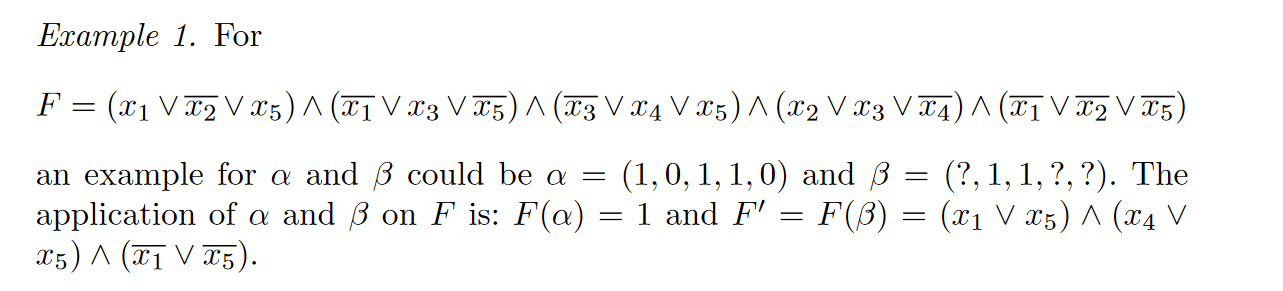
\includegraphics[width=1\linewidth]{1.png}
	\end{figure}
\end{frame}

\begin{frame}
	\frametitle{Some definition}
	\begin{figure}[htbp]
		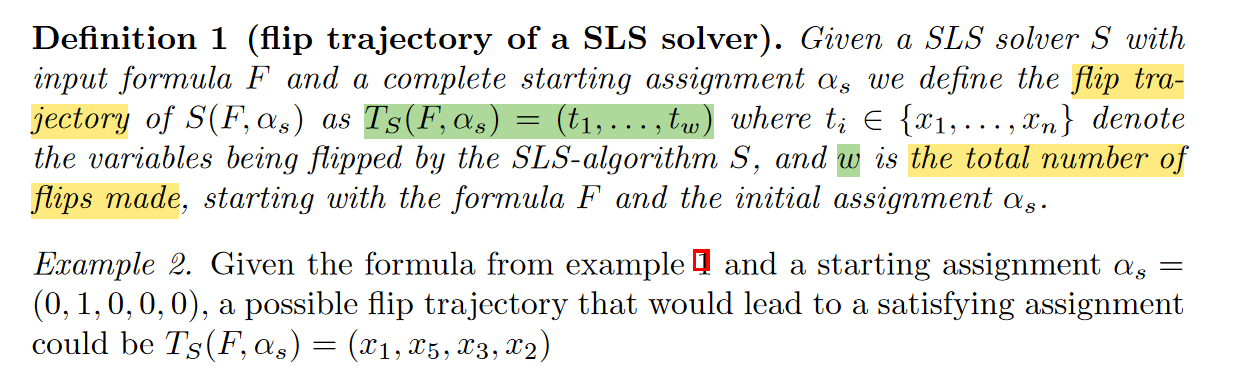
\includegraphics[width=1\linewidth]{2.png}
	\end{figure}
\end{frame}

\begin{frame}
	\frametitle{Some definition}
	\begin{figure}[htbp]
		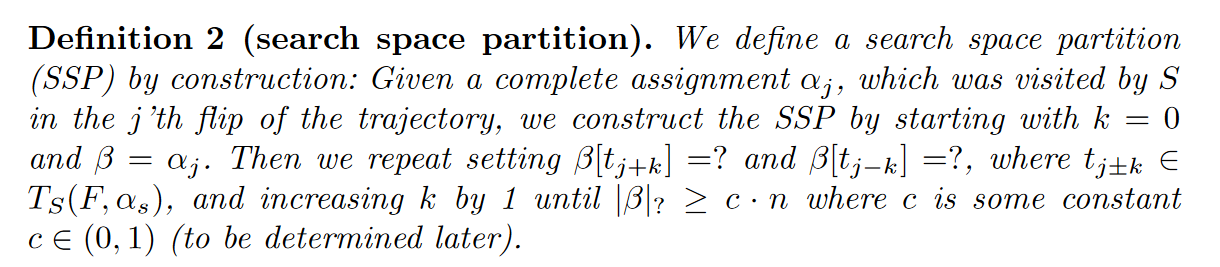
\includegraphics[width=1\linewidth]{3.png}
	\end{figure}
\end{frame}

\begin{frame}
	\frametitle{Some definition}
	\begin{figure}[htbp]
		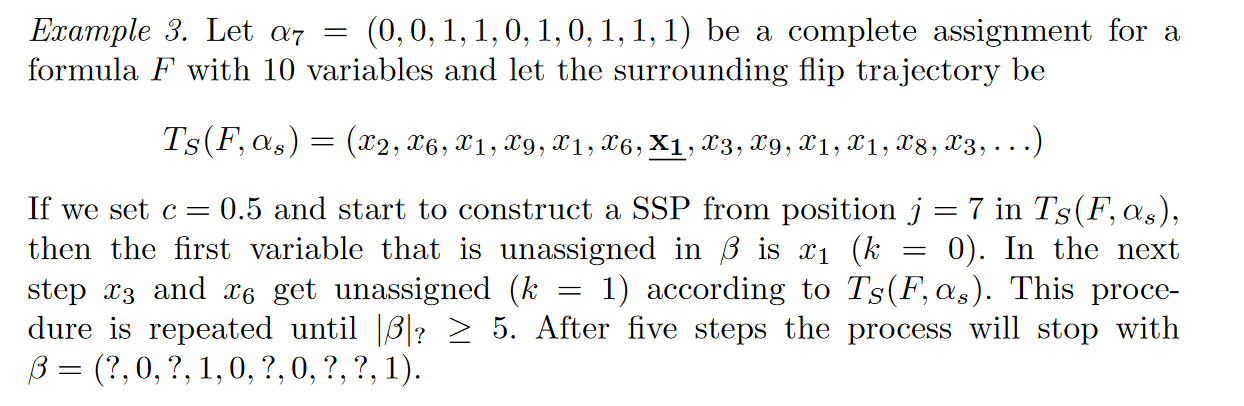
\includegraphics[width=1\linewidth]{4.png}
	\end{figure}
\end{frame}

% \begin{frame}
% 	\frametitle{Use of Search Space Partitions}
% 	\begin{figure}[htbp]
% 		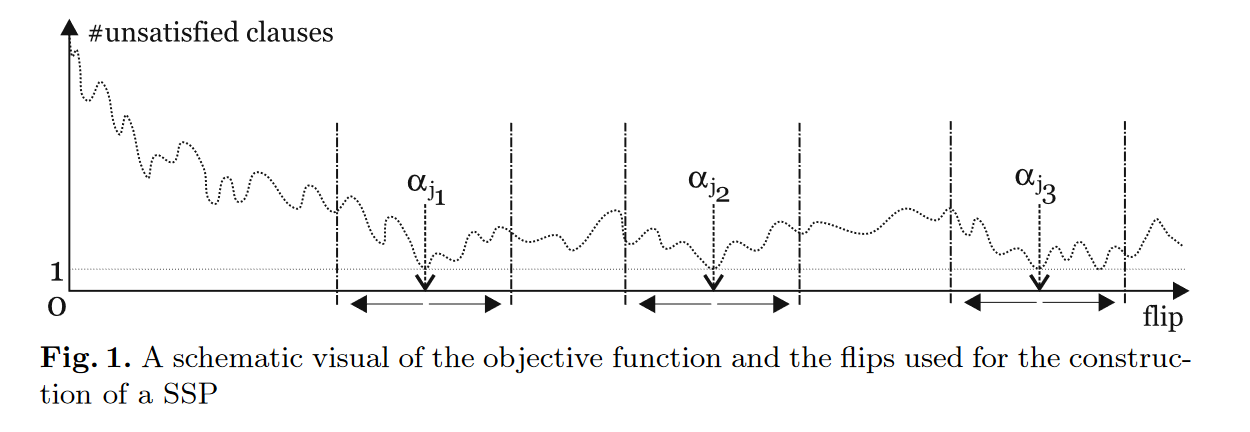
\includegraphics[width=1\linewidth]{5.png}
% 	\end{figure}
% \end{frame}

\begin{frame}
	\frametitle{Use of Search Space Partitions}
	\begin{columns}
		\begin{column}{.45\textwidth}
			\begin{itemize}
				\item SSP can contain multiple minima
				\item Monitoring the flips made by the SLS solver around the discovered local minimum in the trajectory
				\item Then,unassigning these identified variables in the complete assignment of the local minimum, and calling DPLL
				\item If DPLL fail, continue to identify a new local minima
			\end{itemize}
		\end{column}

		\begin{column}{.55\textwidth}
			\begin{figure}[htbp]
				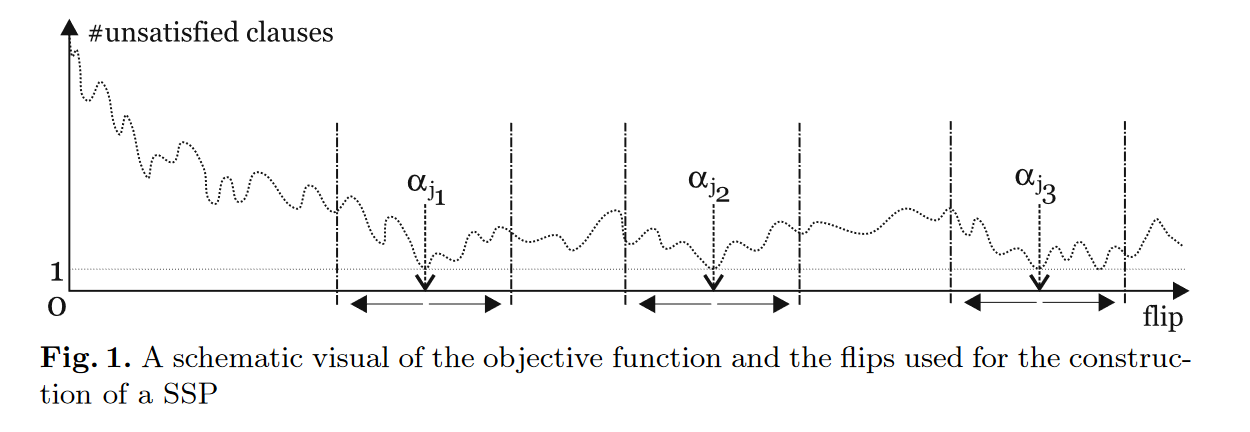
\includegraphics[width=1\linewidth]{5.png}
			\end{figure}
		\end{column}
	\end{columns}
\end{frame}

\begin{frame}
	\frametitle{Use of Search Space Partitions}
	\begin{figure}[htbp]
		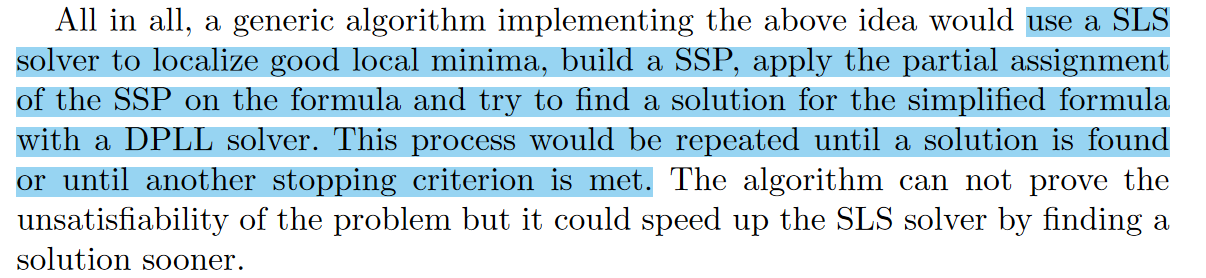
\includegraphics[width=1\linewidth]{6.png}
	\end{figure}
\end{frame}

\section{hybridGM}
\begin{frame}
	\frametitle{Pseudocode for hybridGM}
	\begin{columns}
		\begin{column}{.5\textwidth}
			\begin{figure}[htbp]
				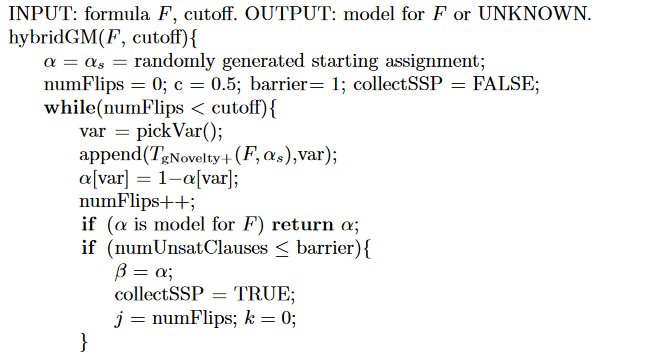
\includegraphics[width=1\linewidth]{7.png}
			\end{figure}
		\end{column}

		\begin{column}{.5\textwidth}
			\begin{figure}[htbp]
				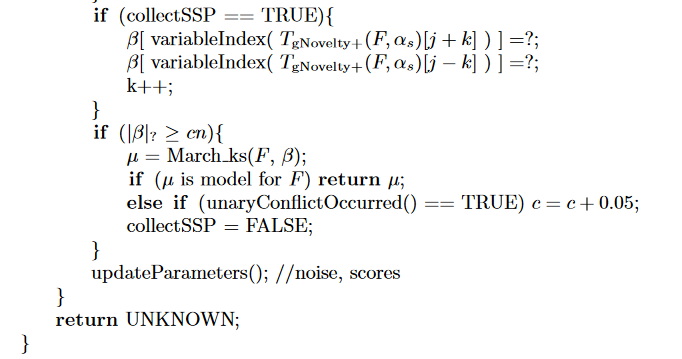
\includegraphics[width=1\linewidth]{8.png}
			\end{figure}
		\end{column}
	\end{columns}


\end{frame}

% \begin{frame}
% 	\begin{tabular}{l|ccccccccc} 
% 						  variable    & $v_{11}$ & $v_{21}^{b}$ & $v_{21}^{f}$ & $v_{22}^{b}$ & $v_{22}^{f}$ & $v_{31}$ & $a_{1}$ & $a_{2}$ & $a_{3}$ \\
% 		\cline { 2 - 10 } lower bound & 0        & $-\infty$    & 0            & $-\infty$    & 0            & $0.5$ & 0 & 0 & 0 \\
% 		\cline { 2 - 10 } assignment  & 0        & 0.5          & 0.5          & 0            & 0            & 0.5  & 0.5 & 0 & 0 \\
% 		\cline { 2 - 10 } upper bound & 1        & $\infty$     & $\infty$     & $\infty$     & $\infty$ & 1 & 0 & 0 & 0
% 	\end{tabular}

% 	\begin{tabular}{l|ccccccccc} 
% 		variable & $v_{11}$ & $v_{21}^{b}$ & $v_{21}^{f}$ & $v_{22}^{b}$ & $v_{22}^{f}$ & $v_{31}$ & $a_{1}$ & $a_{2}$ & $a_{3}$ \\
% 		\cline { 2 - 10 } lower bound & 0 & $-\infty$ & 0 & $-\infty$ & 0 & $0.5$ & 0 & 0 & 0 \\
% 		\cline { 2 - 10 } assignment & 0.5 & 0.5 & 0.5 & 0 & 0 & 0.5 & 0 & 0.5 & 0 \\
% 		\cline { 2 - 10 } upper bound & 1 & $\infty$ & $\infty$ & $\infty$ & $\infty$ & 1 & 0 & 0 & 0
% 	\end{tabular}

% \end{frame}

% \begin{frame}
% 	\begin{tabular}{c|ccccccccc}
% 		$\mathrm{T}$  & $p$  & $q$ & $r$ & $s$ & $t$ &   & $\mathrm{Ib}$ & $\beta$ & $u b$ \\
% 		\hline$x$     & $-2$ & 1   &     &     &         & 0             & $-1$    & 0 \\
% 		$y$           &      & 1   & 2   &     &         & 0             & 0       & 0 \\
% 		$z$ & & & $-1$ & 1 & 1 & 0 & 0 & 0 \\
% 		$u b$ & 1 & $+\infty$ & $+\infty$ & $+\infty$ & $+\infty$ & & & \\
% 		$\alpha$ & $0.5$ & 0 & 0 & 0 & 0 & & & \\
% 		$\mathrm{lb}$ & $0.5$ & $-\infty$ & $-\infty$ & 0 & 0 & & Simplex
% 		\end{tabular}
% \end{frame}


\section{Conclusions and Future Work}

\begin{frame}
	\frametitle{Conclusions}
	\begin{itemize}
		\item We defined this new term SSP, explained how such SSPs are constructed and how they are used.
		\item We implemented our novel approach in the hybrid SAT solver \emph{hybridGM}, utilizing \emph{gNovelty+} as the SLS component and \emph{March\_ks} as the DPLL component.
	\end{itemize}
\end{frame}

\begin{frame}
	\frametitle{Future Work}
	\begin{itemize}
		\item On uniform random 5- and 7-SAT instances, March ks almost never finds a solution.
		\item Dynamically adapt the barrier while hybridGM performs a search.
	\end{itemize}
\end{frame}

%------------------------------------------------


%------------------------------------------------

%------------------------------------------------


%------------------------------------------------
\begin{frame}
\hfill
\center{\Huge{\calligra{\Huge{Thank you}}}}
\linespread{3}\selectfont
\end{frame}
%----------------------------------------------------------------------------------------
\end{document}